\documentclass[tikz]{standalone}

\usepackage{quantumcircuit}
\usetikzlibrary{positioning}
\usepackage{pgfplots}
\pgfplotsset{compat=1.17}

\begin{document}
\begin{tikzpicture}
  \let\qmwires\empty
  % define initial positions of the quantum wires
  \xdef\dy{0.85}
  \defwire (S) at ({-\dy});
  \defwire (D1) at ({-2*\dy});
  \defwire (D2) at ({-3*\dy});
  \defwire (D3) at ({-4*\dy});
  \defwire (D4) at ({-5*\dy});
  % draw wires
  \xdef\dt{1}
  \drawwires [\dt] (8);
  
  % Draw gates
  \gate (S-0) [$R_X$];
  \cnot (S-4) (D3-4);
  \cnot (S-5) (D4-5);
  \gate (S-8) [$M_X$];
  
  % Draw outputs/inputs
  % \node[xshift=-2em]  at ($(D1-0)!0.5!(D4-0)$) {$\ket{\psi}$};
\end{tikzpicture}
\end{document}

%%% Local Variables:
%%% coding: utf-8
%%% TeX-master: t
%%% TeX-command-extra-options: "-shell-escape"
%%% End:
